\section{The model}
\label{sec:modelDescription}

The inequality trading model consists of an economy with $N$ agents, each with wealth $c_i$ with $ i = 1, \ldots, N$. Agents are allowed to trade among themselves $M$ objects, with each object $m = 1, \ldots,M$ having a price $\pi_m$. A given allocation of goods among the agents is described by an $N\times M$ allocation matrix $\mathcal{A}$ with entries $a_{i,m} = 1$ if agent $i$ owns good $m$ and zero otherwise. Agents can only own baskets of goods that they can afford, i.e. whose total value does not exceed their wealth. The wealth not invested in goods
\begin{equation}
c_i -  \sum_{m=1}^M a_{i , m} \pi_m =\ell_i\ge 0, \quad\quad i=1,\ldots,N,
\label{eq:1}
\end{equation}
corresponds to the cash (liquid capital) that agent $i$ has available for trading.  Therefore 
the set of feasible allocations -- those for which $\ell_i\ge 0$ for all $i$ -- is only a small fraction of the $M^N$ conceivable allocation matrices $\mathcal{A}$.

Starting from a feasible allocation matrix $\mathcal{A}$, we introduce a random trading dynamics in which a good $m$ is picked uniformly at random among all goods. Its owner then attempts to sell it to another agent $i$ drawn uniformly at random among the other agents. If agent $i$ has enough cash to buy the product $m$, that is if $\ell_i \ge \pi_m$, the transaction is successful and his/her cash decreases by $\pi_m$ while the cash of the seller increases by $\pi_m$, otherwise the transaction fails, with no possibility of an object being divided. Notice that the total capital $c_i$ of agents does not change over time, so $c_i$ and the prices $\pi_m$ are parameters of the model. The entries of the allocation matrix, and consequently the cash, are dynamical variables, which evolve over time according to this dynamics. This model belongs to the class of zero-intelligent agent-based models, because agents do not try to maximize any utility function and simply trade the goods they have at random.

A crucial property of the dynamic described above is that the stochastic transition matrix $W(\mathcal{A}\to\mathcal{A}')$ is symmetric between any two feasible configurations $\mathcal{A}$ and $\mathcal{A}'$: $W(\mathcal{A}\to \mathcal{A}')=W(\mathcal{A}'\to \mathcal{A})$. Note that any feasible allocation $\mathcal{A}$ can be reached from any other feasible allocation $\mathcal{A}'$ by a sequence of trades. This implies that the dynamic satisfies the detailed balance condition:

\begin{align}
W(\mathcal{A} \to \mathcal{A}') P(\mathcal{A}) = W(\mathcal{A}'\to \mathcal{A})P(\mathcal{A}'),  \quad \forall \mathcal{A}, \mathcal{A}'
\end{align}
with a stationary distribution over the space of feasible configurations that is uniform, ie, $P(\mathcal{A})= \text{const}$. This is consequence of the symmetric transition rates, and would be the same for every trading rule that has $W(\mathcal{A}\to \mathcal{A}')=W(\mathcal{A}'\to \mathcal{A})$. In fact, the current trading rules employed in this model are a particular case of a general rule for which we first select a subset of $n$ agents, $2 \leq n \leq N$, then we pick a random good from these $n$ agents and try to trade it with the remaining $n-1$ agents, automatically accepting if the chosen buyer has enough cash to purchase it. This rule may sound cryptic, but it's common in the particular cases of $n=N$, which is the current one described in the model, and for $n=2$, in which we first pick two consumers and then try to exchange a random good among themselves. All of these rules generate the same stationary distribution.

The analysis presented here is restricted to symmetric rates because otherwise, even if we held detailed balance, we would have to explicitly find the probability density over the configurations. Since the resulting density would be non-uniform, it would be more difficult to link dynamical observables (rate of money transfer, etc.) to static variables (number of neighbouring configuration to a given configuration). We do not explore these cases.

These rules are not the only ones providing symmetric rates, or even that this property is necessary for interesting dynamics. We simply point out that the detail of the choice of the dynamical rule is not crucial, as long as we as we have a simple zero-intelligent dynamics which generates symmetric transition rates. We now give a few examples of rules that are either identical to those above, or do not yield symmetrical probabilities of transfer:


For the intial agent's capital, we choose to focus on realisations where the wealth $c_i$ is drawn from a Pareto distribution $P\{c_i> c\} \sim c^{-\beta}$, for $c>c_{\min}$ for each agent $i$, which is compatible with many empirical observations of real world wealth distribution. We allow $\beta$ to vary so that we are able to explore different levels of inequality, and compare different economies in which the ratio between the total wealth $C=\sum_i c_i$ and the total value of all objects $\Pi=\sum_{m}\pi_m$ is kept fixed. We use $C>\Pi$ so as to have feasible allocations.

For the goods, we are going to limit the analysis to cases where the $M$ objects are divided into a small number of $K$ classes with $M_k$ objects per class ($k=1,\ldots,K$), objects belonging to class $k$ have the same price $\pi_{(k)}$. If $z_{i,k}$ is the number of object of class $k$ that agent $i$ owns, then \eqref{eq:1} takes the form

\begin{equation}
c_i =  \sum_{k=1}^K z_{i , k} \pi_{(k)} + \ell_i
\end{equation}

In the next section we will solve the master equation and find the distribution of goods as a function of capital $c_i$. As it will be shown, the main result of this model is that the flow of goods among agents becomes more and more congested as inequality increases until it halts completely when the Pareto exponent $\beta$ tends to one.


\section{The case of one good}

We begin our analysis by the simplest case in which there is only one type of good being traded, ie, $K=1$, but the results shown will extend for the general setting. A formal approach to this problem consists in writing the complete Master Equation that describes the evolution of the probability $P(z_1,\ldots, z_N)$ of finding the economy in a state where each agent $i=1,\ldots,N$ has a specific number $z_i$ of goods. Taking the sum over all values of $z_j$ for $j\neq i$, one can derive the Master Equation for a single agent with wealth $c_i$. The corresponding marginal distribution $P_i(z)$ in the stationary state can be derived from the detailed balance condition

\begin{equation}
P_i(z+1)  \frac{z+1}{M}  p^s =  P_i(z) \frac{1}{N} \left(1-\delta_{z, m_{i}}\right) ,\qquad z=0,1,\ldots, m_i
\label{Eq:MasterEq3_1Good_1Guy}
\end{equation}
where $m_{i}=\floor{c_i / \pi}$ is the maximum number of goods which agent $i$ can buy with wealth $c_i$ and $p^{s}$ is the probability that a transaction where agent $i$ sells one good (i.e. $z+1\to z$) is successful. Equation \eqref{Eq:MasterEq3_1Good_1Guy} says that, in the stationary state, the probability that agent $i$ has $z$ objects and buys a new object is equal to the probability to have agent $i$ with $z+1$ objects and successfully selling one of them. The factor $1-\delta_{z, m_{i}}$ enforces the condition that agent $i$ can afford at most $m_i$ goods and it implies that $P_i(z)=0$ for $z>m_i$. Exchanges are successful if the buyer $j$ does not already have a saturated budget $z_j=m_j$. So the probability of success $p^s$ for the trade is given by

\begin{align}
p^s & =  1-\frac{1}{N-1}\sum_{j\neq i} P\{z_j=m_j|z_i=z\}\\
 & \cong  1-\frac{1}{N}\sum_{j} P_j(m_j)\qquad (N,M\gg 1)\label{eq:ps_1Guy}
\end{align}
where the last relation holds because when $N,M\gg 1$ the dependence on $z$ becomes negligible. This is important because it implies that for large $N$ the variables $z_i$ can be considered as independent, i.e., $P(z_1,\ldots, z_N)=\prod_i P_i(z_i)$, and the problem can be reduced to that of computing properties from the marginals $P_i(z_i)$.

One probability distribution that solves equation \eqref{Eq:MasterEq3_1Good_1Guy} is a truncated Poisson distribution with parameter $\lambda = M / (N p^s) $:

\begin{equation}
P_i(z) = \frac{1}{Z_i} \left[ \frac{\lambda^{z}}{z!}\right] \Theta\left(m_i - z \right),
\label{Eq:ME_solution_1Good}
\end{equation}
where $Z_i$ is a normalization factor that can be determined by $\sum_{z} P_i(z) = 1$. Finally, the value of $p^s$ -- or equivalently of $\lambda$ -- can be found self-consistently, by solving equation \eqref{eq:ps_1Guy}, which we will show in the next section.

From the stationarity distribution \eqref{Eq:ME_solution_1Good}, we see that the most likely value of $z$ for an agent with $m_i=m$ is given by

\begin{equation}
z^\ast(m)  = \argmax_z  P(z)=
\begin{cases}
    m, & \text{ if } m \leq \lambda \\
    \lambda, & \text{ if } \lambda \leq m
  \end{cases}.
  \label{Eq:cases_ztyp}
\end{equation}

This provides a natural distinction between cash-poor agents -- those with $m \leq \lambda$ --  that often cannot afford to buy any other object, and cash-rich ones -- those with $m> \lambda$ --  who typically have enough cash to buy further objects. We simulate the model with one good and compare the goods distribution after equilibrium against the theoretical predicted, the results are shown in figure \ref{Fig:Picturesque_RichPoor_transition_beta}. We can indeed these two types of agents in the simulations, which agree very well with the theoretical prediction. The inset of figure \ref{Fig:Picturesque_RichPoor_transition_beta} shows the cash distribution $P_i(\ell/\pi)$ (where $\ell/\pi = c_i/\pi - z$ represents the number of goods they are able to buy) for some representative agents. While cash-poor agents have a cash distribution peaked at $0$, the wealthiest agents have cash in abundance.

\begin{figure}%[htbp!]
\centering
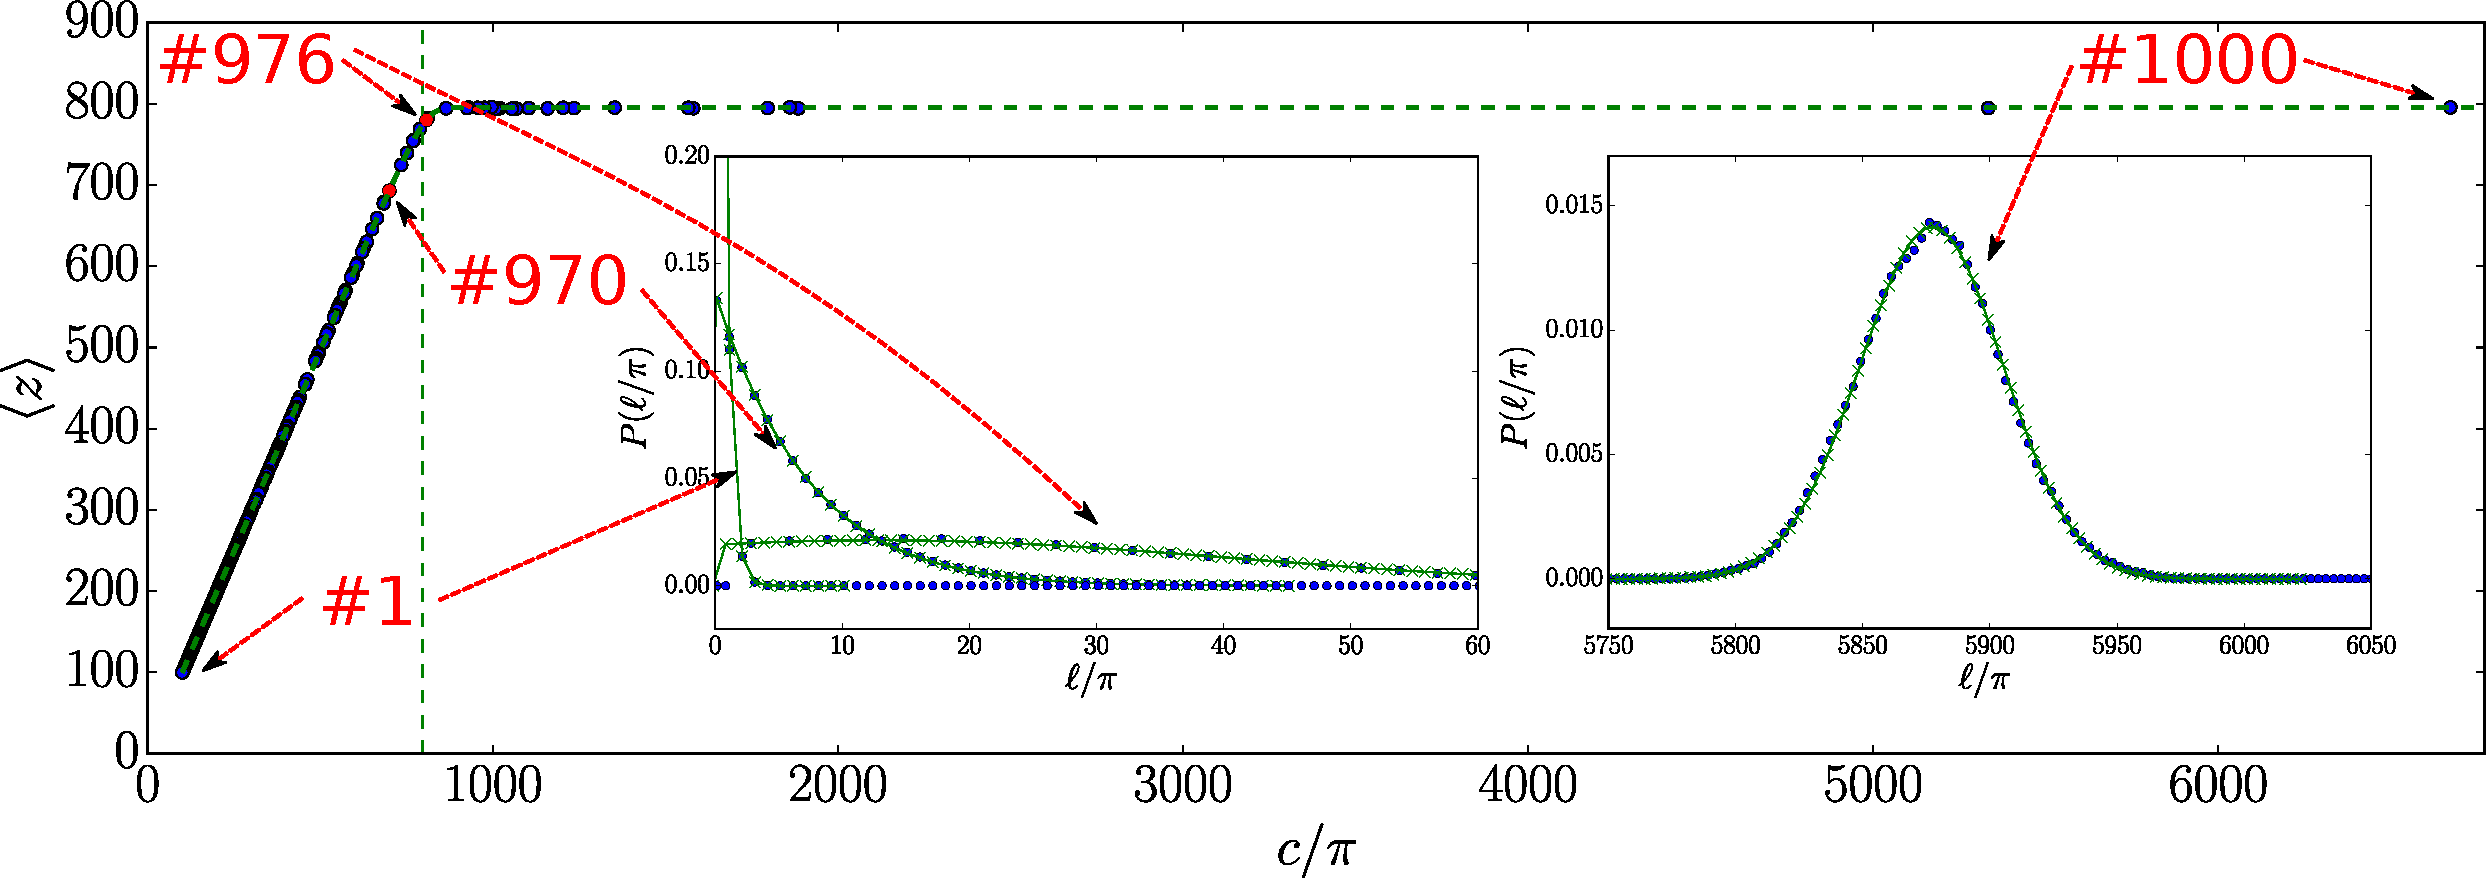
\includegraphics[width=\textwidth]{figs_ineq/fig3_ownership_average_beta=1p80_e=1p10-byHand.pdf}
\caption{\textbf{(Main)} Average number of owned goods in an economy with a single type of good, $N=10^3$ agents, $\beta=1.8$, $M\approx 2 . 10^5$ and $C/\Pi=1.1$. Points $\{(\langle z \rangle_i,c_i)\}_{i=1}^{N}$ denote the average composition of capital for different agents obtained in Monte Carlo simulations, compared with the analytical solution obtained from the Master Equation (green dashed line) given by equation \eqref{Eq:ME_solution_1Good}.
The vertical dashed line at $c^{(1)}\simeq 7.98=M/N p^s_1$ indicates the analytically predicted value of the crossover wealth that separates the two classes of agents. \textbf{(Insets)} Cash distributions $P_i(\ell)$ of the indicated agents. 
}
\label{Fig:Picturesque_RichPoor_transition_beta}
\end{figure}

In terms of wealth, the poor are defined as those with $c_i<c^{(1)}$ whereas the rich ones have $c_i>c^{(1)}$, where the threshold wealth is given by 

\begin{equation}
c^{(1)} = \lambda \pi = M \pi/(N p^s)
\label{eq:c1}
\end{equation}

Notice that when $\lambda\gg 1$, a condition that occurs when the economy is nearly frozen ($p^s\ll 1$), the distribution $P_i(z)$ is sharply peaked around $z^{\text{mode}}(m)$ so that its average is $\langle z\rangle\simeq z^{\text{mode}}(m)$. Then the separation between the two classes becomes rather sharp, as in Figure \ref{Fig:Picturesque_RichPoor_transition_beta}.

We can compute $p^s$ by using equation \eqref{eq:ps_1Guy}, $p^s = 1 - \frac{1}{N} \sum_{i=1}^{N} P_i(z = m_i)$, and approximating the probability to be on a threshold $P_i(z=m_i)$ by

\begin{align}
P_i(z=m_i) = 
\begin{cases}
\left( 1 - \frac{m_i}{\lambda} \right) & \text{ for } m_i \ll \lambda \\
0 & \text{ for } m_i > \lambda
\end{cases}.
\end{align}

The first case can be understood by noting that in the limit $m_i \ll \lambda$ we have the approximation

\begin{equation}
P_i(z=m_i) = \frac{\lambda^{m_i} \frac{1}{m_i!}}{\sum_{x=0}^{m_i} \lambda^x \frac{1}{x!}} = \frac{1}{1 + \frac{m_i}{\lambda} + \frac{m_i (m_i -1)}{\lambda^2} + \ldots} \simeq  \left( 1 - \frac{m_i}{\lambda} \right),
\end{equation}

Assuming this approximation to be valid for all $m_i < \lambda$ is clearly a bad assumption for all agents with $m_i$ close to $\lambda$. 
However the wealth is power law distributed, and so the weight of agents with $m_i \sim \lambda$ is negligible in the sum over all agents in equation \eqref{eq:app_ps_analytic0}. The accuracy of this approximation increases when the exponent of the power law $\beta$ decreases. 

$p^s$ can then be computed using

\begin{equation}
\label{eq:app_ps_analytic1}
p^s = 1 - \frac{1}{N} \sum_{i=1}^{N} P_i(z = m_i) \simeq 1 - \int_1^{c^{(1)} = \lambda \pi} dc\, \beta c^{-\beta - 1} \left( 1 - \frac{c}{\lambda \pi} \right) .
\end{equation}

This is an implicit expression for $p^s$, since it appears on the left hand side of the equation and also inside the integral, because $\lambda = \frac{M}{N p^s}$, which makes it untractable to solve analytically. 

There are two approximations we can use to solve this equation: the first and most straightforward is to assume that $\lambda$ can be replaced by its expected value on the realizations, i.e., $M/N$ is a random variable that depends on the realization of the capital distribution due to the fixed constant $\Pi/C$.  We replace $M$ by it's expected value, $\Pi/\pi$ and $N$ by $C / \langle c \rangle$, where $\langle c \rangle$ is the expected capital per agent, which is given by the average of the beta distribution, $\langle c \rangle = \beta/(\beta-1)$. For finite $N$, this is only a reasonable approximation if $\beta \gg 1$, and breaks down in the limit $\beta \to 1^+$ due to the infinite variance of the capital distribution, but it should be accurate for all $\beta > 1$ in the limit $N \to \infty$. Using the approximation on \eqref{eq:c1} and replacing $\lambda = c^{(1)} / \pi$, we have:

\begin{equation}
\frac{M}{N \lambda} \to \left \langle \frac{M}{N} \right \rangle \frac{\pi}{c^{(1)}} = \frac{\Pi}{C} \frac{\beta}{\beta - 1} \frac{1}{c^{(1)}}
\end{equation}

So we have

\begin{equation}
 \label{Eq:ps_correct}
p^s = \frac{M}{N \lambda} = \frac{\Pi}{C} \frac{\langle c \rangle}{c^{(1)}},
\end{equation} 
which gives us $p^s$ but as a function of $c^{(1)}$, which we don't know. But now that this is independent of $p^s$, we can put this expression back into $\eqref{eq:app_ps_analytic1}$ and carry out the integration to get an analytic form for $c^{(1)}$:

\begin{equation}
\frac{\Pi}{C} \frac{\langle c \rangle}{c^{(1)}} = {c^{(1)}}^{-\beta} \left( \frac{1}{1-\beta} \right) - \frac{\beta}{1 - \beta } \frac{1}{c^{(1)}},
\end{equation}

Solving for $c^{(1)}$ we have

\begin{equation}
\label{Eq:c1_correct}
c^{(1)} = \left[\beta \left(  1 - \frac{\Pi}{C}\right) \right]^{1/(1 - \beta)}.
\end{equation}

And replacing this back on equation \eqref{Eq:ps_correct} gives $p_s$ as a function of the intensive variables for the economy

\begin{equation}
p^s = \frac{\Pi}{C}\frac{\beta}{\beta - 1} \frac{1}{\left[\beta \left(1 - \frac{\Pi}{C}\right) \right]^{1/(1 - \beta)}}.
\end{equation}

Notice that $\langle c \rangle$ diverges as $\beta \to 1^+$, but also that within this approximation the threshold wealth $c^{(1)}$ diverges much faster, with an essential singularity. More precisely, we note that $\Pi/C<1$, so that $\beta ( 1- \Pi/C) \sim (1-\Pi/C)$ is a number smaller than 1 (yet positive). From equation \eqref{Eq:c1_correct}, we have $c^{(1)}\sim (1-\Pi/C)^{-1/(\beta-1)} \to \infty$ and therefore the liquidity $p^s$ vanishes as $\beta \to 1^+$. 

For finite $N$, this approximation breaks down when $\beta$ gets too close to or smaller than one, because $\langle c \rangle$ is ill-defined and in equation \eqref{Eq:ps_correct} it should be replaced with $1/N \sum_i c_i $, which strongly fluctuates between realizations and depends on $N$. An estimate of $p^s$ for finite $N$ and $\beta<1$ can be obtained by observing that the wealth $c^{(1)}$ that marks the separation between the two classes cannot be larger than the wealth $c_{\max}$ of the wealthiest agent. By extreme value theory, the latter is given by $c_{\max}\sim N^{1/\beta}$, with $a>0$. Therefore the solution is characterised by $ c^{(1)}=\pi \lambda\sim c_{\max}\sim N^{1/\beta}$. Furthermore, for $\beta<1$ the average wealth is dominated by the wealthiest few, i.e. $\langle c \rangle \sim N^{1/\beta-1}$ and therefore  $p^s \sim N^{1/\beta-1}/c^{(1)} \sim N^{-1}$. In other words, in this limit the cash-rich class is composed of a finite number of agents, who hold almost all the cash of the economy. However, as we show in figure \ref{Fig:ps_one_good} the above rough analytical estimate of $p_s$ is in good agreement with the numerical simulations.

% TODO: explain iterative method
\begin{figure}
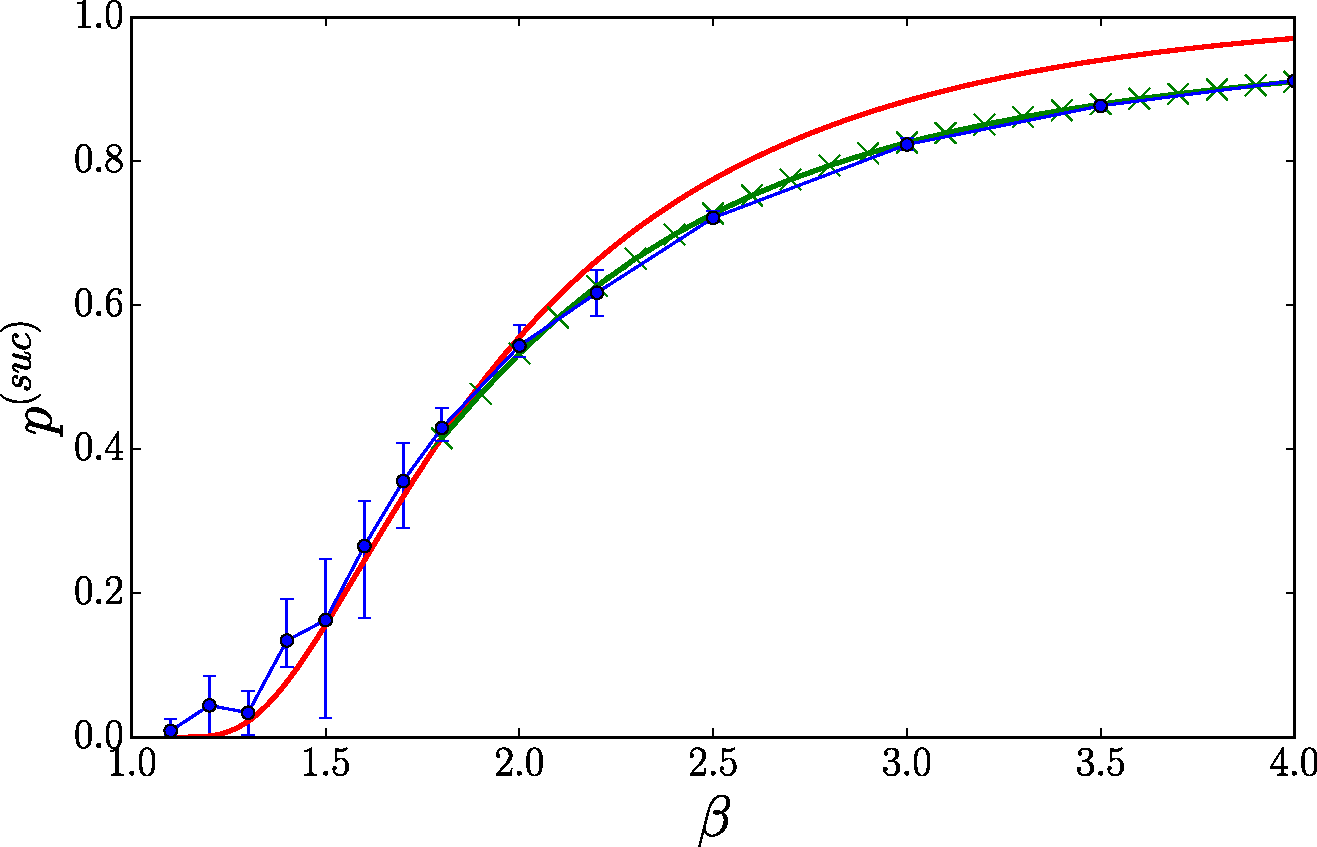
\includegraphics[width=\textwidth]{figs_ineq/fig_K=1_e=1p2_g=undef_ps_prediction_unadj.pdf}
\caption{Comparison between numerical simulations and analytical estimates for the success probability of transaction $p^s$ for one class of goods, as a function of the Pareto exponent $\beta$. The blue solid circles are the result  of Monte Carlo simulations performed for $N=10^5$ agents and averaged over 5 realizations, with the error bars indicating the min and max value of $p^s$ over all realizations. The red lines are the analytic estimates  according to equation \eqref{Eq:ps_correct}. The green crossed lines correspond to numerically solving the analytical solution  \eqref{Eq:ME_solution_2Goods} for a population composed of $N=64$ "agents".
}
\label{Fig:ps_one_good}
\end{figure}


\section{The general case}

The analysis presented in the last section carries over to the general case in which $K$ classes of goods are considered, starting from the full Master Equation for the joint probability of the ownership vectors $\vec z_i=(z_{i,1}\ldots, z_{i,K})$ for all agents $i=1,\ldots,N$. For the same reasons as before, the problem can be reduced to that of computing the marginal distribution $P_i(\vec z_i)$ of a single agent. The main complication is that the maximum number $m_{i,k}$ of goods of class $k$ that agent $i$ can get now depends on how many of the other goods agent $i$ owns, i.e. $m_{i,k}(z^{(k)}_i)=\floor{(c_i-\sum_{k'(\neq k)} z_{i,k'} \pi_{(k')})/\pi_{{k}}}$, where $z^{(k)}_i=\{z_{i,{k'}}\}_{k'(\neq k)}$. The detailed balance condition is

\begin{equation}
\label{Eq:MasterEq3_2Goods_1Guy}
P_i(\vec z+\hat e_k)\frac{z_k+1}{M}p^s_{k}=
P_i(\vec z)  \frac{M_k}{M} \frac{1}{N} \left(1-\delta_{z_k,m_{i,k}(z_{(k)})}\right) 
\end{equation}

In this equation $\hat e_k$ is the vector with all zero components and with a $k^{\rm th}$ component equal to one and $p^s_{k}$ is the probability that a sale of an object of type $k$ is successful. This detailed balance condition again yields the stationary state distribution for $N,M\gg 1$. On the left we have the probability that one of the $z_k+1$ objects of type $k$ of agent $i$ is picked for a successful sale. This must balance the probability (on the r.h.s.) that agent $i$ is selected as the buyer of an object of type $k$, which requires that agent $i$ has less than $m_{i,k}(z_{(k)})$ objects of type $k$, for the transaction to occur (here $M_k/M$ is the probability that an object of type $k$ is picked at random, and $1/N$ is the probability that agent $i$ is selected as the buyer). It can easily be checked that the solution to this set of equations is given by a product of Poisson distributions with parameters $\lambda_k=M_k/(N p^s_{k})$, with the constraint given by equation \eqref{eq:1}

\begin{equation}
P_i(z_1,..., z_{K}) = \frac{1}{Z_i} \left[ \prod_{k=1}^{K}\frac{\lambda^{z_k}_k}{z_k!}\right] \Theta\left(c_i - \sum_k^{K} z_k \pi_{(k)}\right)\,,
\label{Eq:ME_solution_2Goods}
\end{equation}
where $Z_i$ is a normalization factor obeying $\sum_{z_1}...  \sum_{z_{K}}  P_i(z_1, ..., z_{K}) = 1$. Here the $p_k^s$ corresponds to the acceptance rates of transactions of goods of class $k$ and are given by

\begin{equation}
p^s_{k} = 1 - \frac{1}{N}\sum_{i=1}^N P\left\{z_{i,k}=m_{i,k}(z_i^{(k)})\right\}\,
\label{eq:ps_Kobjs}
\end{equation}

As in the case with $K = 1$, the values for the probabilities $p^s_{k}$ need to be found heuristically, which can be complicated when $K$ and $M$ are large.

When the total number of objects per agent is large for any class $k$, we expect that $\lambda_1, ..., \lambda_K \gg 1$, and then the values of $z_{i,k}$ are close to their expected values. This implies that the population of agents splits into $K$ classes, where agents with wealth $c_i\in [c^{(k-1)},c^{(k)}]$ have their budget saturated with goods of class $k'\leq k$ and cannot afford more expensive objects (here $c^{(k)}=\lambda_k\pi_{(k)}$, $k=1,\ldots, K$ and $c^{(0)}=c_{\min}$). An estimate for the thresholds $c^{(k)}$ can be derived following the same arguments as for the case of a single type of good, $K=1$, by observing that when analysing the dynamics of goods of type $k$, all agents in class $k'<k$ are effectively frozen and can be neglected.

In the limit  $\beta \to 1^+$ of large inequality, close inspection\footnote{Note that the term in square brackets is smaller than one, when $\beta \to 1^+$.} of equation  \eqref{Eq:ps_and_ck_generalCaseAnyMathcalM1} shows that $ c^{(k)}  \to \infty, \forall k$, 
which implies that all agents become cash-starved except for the wealthiest few. Since $p^s_{k}\sim \langle c \rangle /c^{(k)}$, this implies that all markets freeze: $p^s_{k}\to 0 , \forall k$.  The arrest of the flow of goods appears to be  extremely robust against all choices of the parameter $\pi_{(k)}$, as $p^s_{1}$ is an upper bound for the other success rates of transactions $p^s_{k}$. These conclusions are fully consistent with the results of extensive numerical simulations (see Figure \ref{Fig:summary_section_one_object}).

\begin{figure}
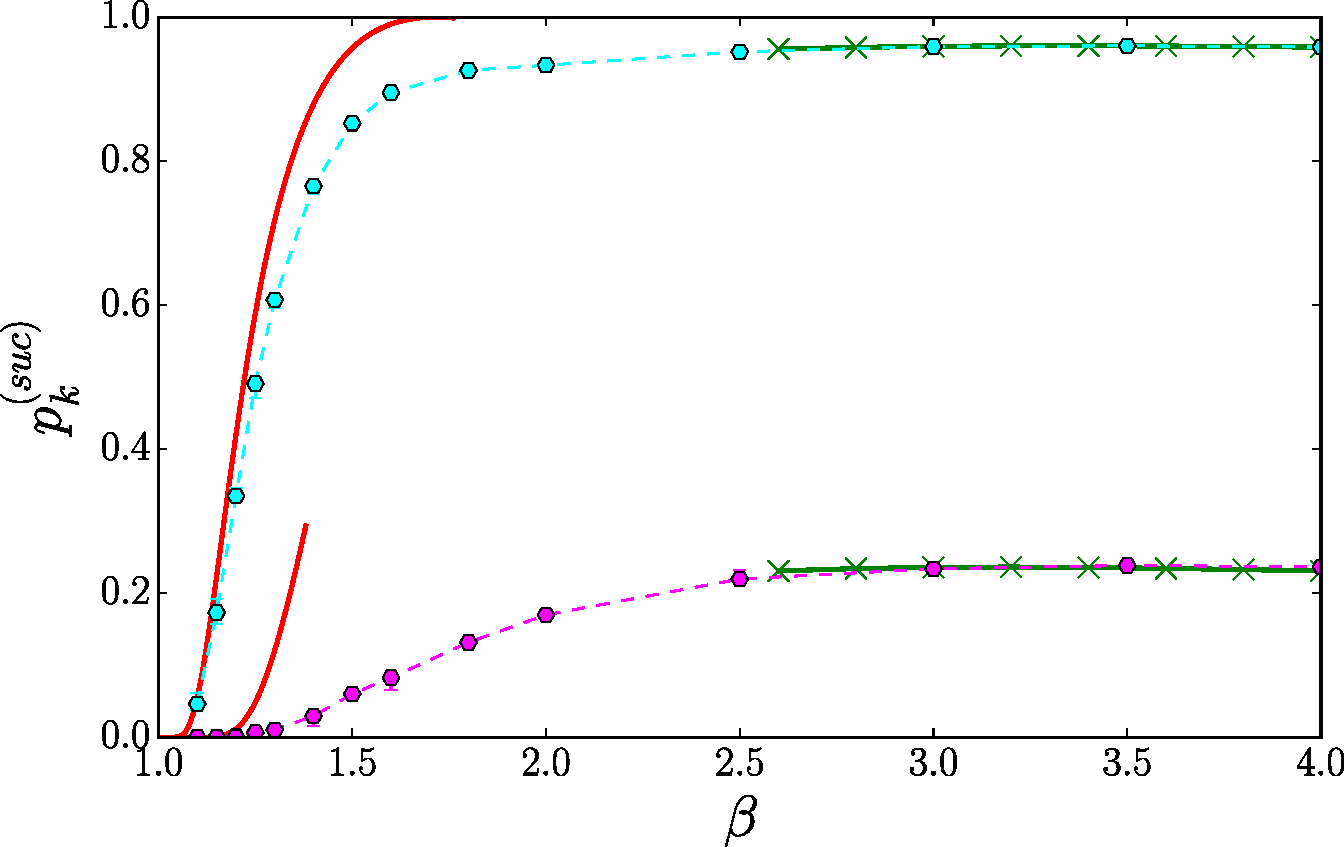
\includegraphics[width=0.8\textwidth]{figs_ineq/fig_K=2_e=1p2_ps_prediction_adjustedcapital.pdf}
\caption{Comparison between numerical simulations and analytical estimates of the success probability of transaction $p^s_k$ for two classes of goods as a function of the Pareto exponent $\beta$. The blue solid circles are the result  of Monte Carlo simulations performed for $N=10^5$ agents and averaged over 5 realizations, with the error bars indicating the min and max value of $p^s_k$ over all realizations. The red lines are the analytic estimates  according to equation \eqref{Eq:ps_and_ck_generalCaseAnyMathcalM1}. The green crossed lines correspond to numerically solving the analytical solution  \eqref{Eq:ME_solution_2Goods} for a population composed of $N=64$ agents.
}
\label{Fig:summary_section_one_object}
\end{figure}

An analytic derivation for the $p_k^s$ and $c^{(k)}$ can be obtained also for the cases of several goods, but only in the limit in which prices are well separated (i.e. $\pi_{(k+1)} \gg \pi_{(k)}$) and the total values of good of any class is approximately constant (we use $M_k\pi_{(k)}  = \Pi / K = {\rm const}$). 
In this limit we expect to find a sharp separation of the population of agents into classes. 
This is because $M_1\gg M_2\gg \ldots \gg M_K$ implies that the market is flooded with objects of the class $1$, which constantly change hands and essentially follow the laws found in the single type of object case. 
On top of this dense gas of objects of class $1$, we can consider objects of class $2$ as a perturbation (they are picked $M_2/M_1$ times less often!).
On the time scale of the dynamics of objects of type $2$, the distribution of cash is such that all agents with a wealth less than $c^{(1)}=\pi_{(1)}\lambda_1$ have their budget saturated by objects of type $1$ and typically do not have enough cash to buy objects of type $2$ nor more expensive ones. 
Likewise, there is a class of agents with $c^{(1)}<c_i\le c^{(2)}$ that will manage to afford goods of types $1$ and $2$, but will hardly ever hold goods more expensive that $\pi_{(2)}$. 

In brief, the economy is segmented into $K$ classes, with class $k$ composed of all agents with  $c_i\in [c^{(k)},c^{(k+1)})$ who can afford objects of class up to $k$, but who are excluded from markets for more expensive goods, because they rarely have enough cash to buy goods more expensive than $\pi_{(k)}$. This structure into classes can be read off from Figure \ref{Fig:K10_ps_beta}, where we present the average cash of agents, given their cash in a specific case (see caption). The horizontal lines denote the prices $\pi_{(k)}$ of the different objects, and the intersections with the horizontal lines define the thresholds $c^{(k)}$. Agents that have $c_i$ just above $c^{(k)}$ are cash-filled in terms of object of class $k$, but are cash-starved in terms of objects $\pi_{(k')}, k'>k$. 

The liquidities $p^s$ can be given by the following expression
\begin{equation}
p^s_{k} = 1 - \frac{1}{N}\sum_{i=1}^N P\left\{z_{i,k}=m_{i,k}(z_i^{(k)})\right\} = 1 - \frac{1}{N}\sum_{i=1}^N P_i(\text{not accepting good type k}) 
\end{equation}
According to the previous discussion of segmentation of the system into $K$ classes, and using the same approximation for this threshold probability discussed in the case of 1 type of good, we assume
\begin{align}
P_i(\text{not accepting good type k}) = 
\begin{cases}
1 & \text{ for } m_i < \lambda_{k-1} \\
\left( 1 - \frac{m_i}{\lambda_k} \right) & \text{ for } \lambda_{k-1} < m_i < \lambda_k \\
0 & \text{ for } m_i > \lambda_k
\end{cases},
\end{align}
Then
\begin{equation}
p^s_{k} \simeq 1 - \int_{1}^{c^{(k-1)}} dc\, \beta c^{-\beta - 1} - \int_{c^{(k-1)}}^{c^{(k)}} dc\, \beta c^{-\beta - 1} \left( 1 - \frac{c}{c^{(k)}} \right) 
\end{equation}
In this case now we have
\begin{equation}
p_k^s = \frac{M_k}{N \lambda_k} = \frac{\Pi}{K C} \frac{\langle c \rangle}{c^{(k)}}
\end{equation}
With similar calculations to the ones showed for the previous case, one can easily get to the recurrence relation:
\begin{equation}
c^{(k)} = \left[ \beta \left( c^{(k-1)} \right)^{1-\beta} - \beta \frac{\Pi}{K C} \right] ^{\frac{1}{1-\beta}}.
\end{equation}
Iterating, we explicit this into: 
\begin{equation}
c^{(k)} = \left[ \beta^k  - \left( \frac{\beta - \beta^{k+1}}{1-\beta} \right) \frac{\Pi}{K C} \right] ^{\frac{1}{1-\beta}},
\end{equation}
 
\begin{align}
c^{(k)} &\simeq \left[ \beta^k  - \left( \frac{\beta - \beta^{k+1}}{1-\beta} \right) \frac{\Pi}{K C} \right] ^{\frac{1}{1-\beta}},
 \label{Eq:ps_and_ck_generalCaseAnyMathcalM1}
\\
p_k^s &= \frac{M_k}{N \lambda_k} \simeq \frac{\Pi}{K C} \frac{\langle c \rangle}{c^{(k)}}.
 \label{Eq:ps_and_ck_generalCaseAnyMathcalM2}
\end{align}



We can also compare the liquid and capital concentrations, measured via their Gini coefficients, for various values of $\beta$ in the system of Fig. \ref{Fig:K10_ps_beta} ($K=10, g=1.5, \pi_{(1)}=0.001, C/\Pi=1.2$).
\begin{figure}%[htbp]
\centering
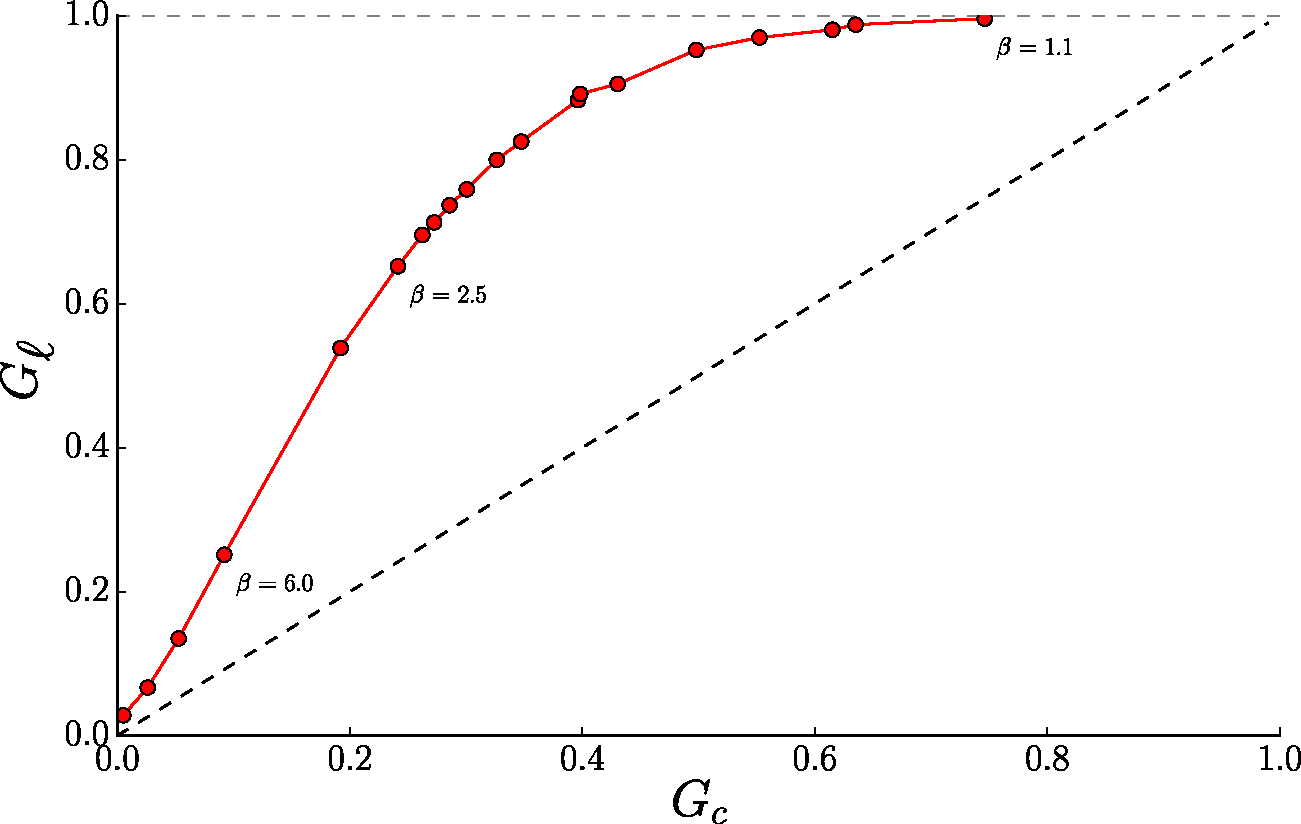
\includegraphics[width=8cm]{figs_ineq/gini_intro.pdf}
\caption{Gini coefficient $G_\ell$ of the cash distribution (liquid capital) in the stationary state of the model as a function of the Gini $G_c$ of the wealth distribution. The dashed line indicates proportionality between cash and wealth, in which case the inequality in both is exactly the same.
The wealth follows a Pareto distribution with exponent $\beta$ that tunes the degree of inequality (the higher is $\beta$, the more egalitarian the distribution).} 
\label{Fig:Gini_Intro}
\end{figure}
In particular, note that the limit $\beta\to 1^+$ is singular, as $G_\ell$ reaches one around $\beta=1.1$, with smaller $\beta$ yielding also $G_\ell\approx 1$.
This is an alternative way to see how the concentration of capital generates an over-concentration of liquidities.

\begin{figure}
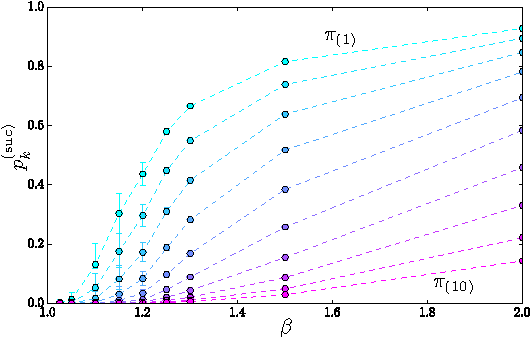
\includegraphics[width=\textwidth]{figs_ineq/cropping-K=10_e=1p2_g=1p5_ps_prediction_adjustedcapital-crop.pdf} \\

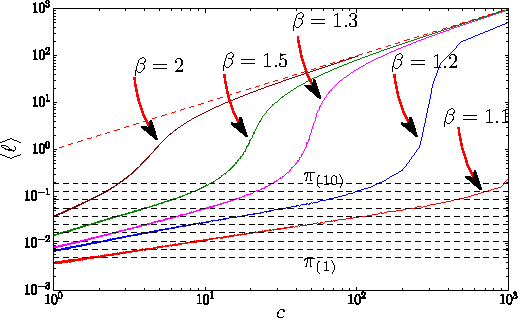
\includegraphics[width=\textwidth]{figs_ineq/cropping-liquidity_global-crop.pdf}
\caption{\textbf{(Top)} Liquidity of goods $\{p^s_k\}_{k=1}^K$  as a function of the inequality exponent $\beta$ for a system of $N=10^5$ agents exchanging $K=10$ classes of goods ($\pi_{(k)}=\pi_{(1)}g^{k-1}$ with $g=1.5$, $\pi_{(1)}=0.005$, $M_k\pi_{(k)}=\Pi/K$ and $C/\Pi=1.2$). Note that all success rates $p^s_k$  vanish when $\beta \to 1^+$.  The curves are ordered from the cheapest (top) to the most expensive (bottom). The markers are the result of numerical simulations, with error bars indicating the minimum and maximum values obtained by averaging over 5 realizations of the wealth allocations. \textbf{(Bottom)} Time averaged cash $\langle \ell_i \rangle$ as a function of wealth $c_i$, from $\beta= 1.1$ to $\beta =2$ for the same simulations with $K=10$ classes of goods. The dashed lines indicate the different prices of goods. Agents with $\langle \ell_i \rangle$ below the price of a good typically have not enough cash to buy it. Cash is proportional to wealth for large levels of wealth (see the upper straight red dashed line). 
}
\label{Fig:K10_ps_beta}
\end{figure}

The decrease of $p^s_k$ when inequality increases (i.e. as $\beta$ decreases) is a consequence of the concentration of cash in the hands of the wealthiest agents. This can be observed in the right panel of  Figure \ref{Fig:K10_ps_beta}, which shows the average cash of agents with a given wealth, for different values of $\beta$. The freezing of the economy when $\beta$ decreases occurs because fewer and fewer agents can dispose of enough cash (i.e. have $\ell > \pi_{(k)}$) to buy the different goods (prices $\pi_{(k)}$ correspond to the dashed lines). 

Note finally that $p^s_k$ quantifies liquidity in terms of goods. In order to have an equivalent measure in terms of cash that can be compared to the velocity of money, we average $\pi_{(k)} p^s_k$ over all goods

\begin{equation}
\label{def:pavg}
\bar p^s=\frac{1}{\Pi}\sum_{k=1}^K M_k \pi_{(k)} p^s_k.
\end{equation}

This quantifies the frequency with which a unit of cash changes hand in our model economy, as a result of a successful transaction. It's behaviour as a function of $\beta$ for the same parameters of the economy in Figure \ref{Fig:K10_ps_beta} is shown in the right panel of Figure \ref{Fig:data}.



\section{Freezing when $\beta \to \infty$.}

 
These two observations allow us to trace the origin of the arrest in the economy back to the shrinkage of the \textit{cash-rich class} to a vanishingly small fraction of the population, as $\beta \to 1^{+}$. As we'll see in the next section, when $\beta$ is smaller than $1$ the fraction of agents belonging to this class vanishes as $N \to \infty$. In this regime, not only the wealthiest few individuals own a finite fraction of the whole economy's wealth, as observed in \cite{bouchaud2000wealth}, but they also drain all the financial resources in the economy.

These findings extend to more complex settings. Figure \ref{Fig:K10_ps_beta} illustrates this for an economy with $K=10$ classes of goods (see figure caption for details) and different values of $\beta$. In order to visualise the freezing of the flow of goods we introduce the success rate of transactions for goods belonging to class $k$, denoted as $p^s_{k}$.  Figure \ref{Fig:K10_ps_beta} shows that, as expected, for a fixed value of the Pareto exponent $\beta$ the success rate increases as the  goods become cheaper, as they are easier to trade.  Secondly it shows that trades of all classes of goods halt as $\beta$ tends to unity, that is when wealth inequality becomes too large, independently of their price.

\section{Conclusions}
\label{sec:con}
In this paper we have introduced a zero-intelligence trading dynamics in which agents have a Pareto distributed  wealth and randomly trade goods with different prices. We have shown that this dynamics leads to a uniform distribution in the space of the allocations that are compatible with the budget constraints.  We have also shown that when the inequality in the distribution of wealth increases, the economy converges to an equilibrium where typically (i.e. with probability very close to one) the less wealthy agents have less and less cash available, as their budget becomes saturated by objects of the cheapest type. At the same time this class of cash-starved agents takes up a larger and larger fraction of the economy, thereby leading to a complete halt of the economy when the distribution of wealth becomes so broad that its expected average diverges (i.e. when $\beta \to 1^{+}$). In these cases, a finite number of the wealthiest agents own almost all the cash of the economy. 

The model presented in this paper is intentionally simple, so as to highlight a simple, robust and quantifiable link between inequality and liquidity. In particular, the model neglects important aspects such as {\em i)} agents' incentives and preferential trading, {\em ii)} endogenous price dynamics and {\em iii)} credit. 
It is worth discussing each of these issues in order to address whether the inclusion of some of these factors would revert our finding that inequality and liquidity are negatively related. 

First, our model assumes that all exchanges that are compatible with budget constraints will take place, but in more realistic setting only exchanges that increase each party's utility should take place. Yet if the economy freezes in the case where agents would accept all exchanges that are compatible with their budget, it should also freeze when only a subset of these exchanges are feasible. Also the model assumes that all agents trade with the same frequency whereas one might expect that rich agents trade more frequently than poorer ones. Could liquidity be restored if trading patterns exhibit some level of homophily, with rich people trading more often and preferentially with rich people? 

First we note that both these effects are already present in our simple setting. Agents with higher wealth are selected more frequently as sellers as they own a larger share of the objects. In spite of the fact that buyers are chosen at random, successful trades occur more frequently when the buyer is wealthy. 
So, in the trades actually observed the wealthier do trade more frequently than the less wealthy, and preferentially with other wealthy agents. 
Furthermore, if agents are allowed to trade only with agents having a similar wealth (e.g. with the $q$ agents immediately wealthier or less wealthy) it is easy to show that detailed balance still holds with the same uniform distribution on allocations. As long as all the states are accessible, the stationary probability distribution remains the same\footnote{
The dynamics changes and thus $p_k^{(\text{suc})}$ changes, in particular for goods more expensive than $\pi_{(1)}$, the seller is typically cash-rich and thus its neighbours are too. This can induce to have a liquidity of expensive goods higher than that of cheaper ones. However in the limit $\beta \to 1^{+}$, it is still true that cash concentrates in the hands of a vanishing fraction of agents, and there is still a freeze of the economy.}. Therefore, our conclusions are robust with respect to a wide range of changes in our basic setting that would account for more realistic trading patterns. 

Secondly, it is reasonable to expect that prices will adjust -- i.e. deflate -- as a result of a diminished demand caused by the lack of liquidity. 
Within our model, the inclusion of price adjustment, occurring on a slower time-scale than trading activity, would reduce the ratio $\Pi/C$ (between total value of goods and total wealth), but it would also change the wealth distribution. 
%If we think of price adjustment as occurring on a slower time-scale than trading activity, this, within our model, would have the effect of reducing the ratio $\Pi/C$ between the total value of goods and the total wealth, but it would also change the wealth distribution. 
Since the freezing phase transition occurs irrespective of the ratio $\Pi/C$, the first effect, though it might alleviate the problem, would not change our main conclusion. The second would make it more compelling, because cash would not depreciate as prices do, so deflation would leave 
wealthy 	% rich 
agents -- who hold most of the cash -- even richer compared to the cash deprived agents, that would suffer the most from deflation. So while price adjustment apparently increases liquidity, this may promote further inequality, that would curtail liquidity further. 

Finally, can the liquidity freeze be avoided by allowing agents to borrow? Access to credit, we believe, will hardly improve the situation\footnote{Allowing agents to borrow using goods as collaterals is equivalent to doubling the
wealth of cash-starved agents, provided that any good can be used only once as a collateral, and that goods bought with credit cannot themselves be used as collaterals.  This would at most blur the crossover between cash-rich agents and cash-starved ones, as intermediate agents would sometimes use credit. This does not change our main conclusion that inequality and liquidity are inversely related and that the economy would halt when $\beta \to 1^{+}$.}, in line with the results in \cite{Yakovenko2009Review} and for similar reasons. Credit may mitigate illiquidity in the short term, but cash deprived agents should borrow from wealthier ones. With positive interest rates, this would make inequality even larger in the long run. So credit is likely to make things worse, in line with the arguments\footnote{Piketty \cite{Piketty2014} observes that when the rate of return on capital exceeds the growth rate of the economy (which is zero in our setting), wealth concentrates more in the hands of the rich.} in \cite{Piketty2014}.

Therefore, even though the model presented here can be enriched in many ways, we don't see a way in which the relation between inequality and liquidity could be reversed. 

Corroborating the present model with empirical data goes beyond the scope of the present paper, yet we remark that our findings are consistent with the recent economic trends, as shown in Figure \ref{Fig:data}.  For example, it is worth observing that, alongside with increasing levels of inequality, trade 
has slowed down after the 2008 crisis\footnote{The {\em U.S. Trade Overview, 2013} of the International Trade Administration observes that ``Historically, exports have grown as a share of U.S. GDP. However, in 2013 exports contributed to 13.5\% of U.S. GDP, a slight drop from 2012'" (see {\tt http://trade.gov/mas/ian/tradestatistics/index.asp{\#P}11}). A similar slowing down can be observed at the global level, in the UNCTAD {\em Trade and Development Report, 2015}, page 7 (see {\tt http://unctad.org/en/pages/PublicationWebflyer.aspx?publicationid=1358}).}. More generally, avoiding deflation -or promoting inflation- has been a major target of monetary policies after 2008, which one could take as an indirect evidence of the slowing down of the economy.  Furthermore, the fact that inequality hampers liquidity and hence promotes demand for credit suggests that the boom in credit market before 2008 and the increasing levels of inequality might not have been a coincidence. 

An interesting side note is that the concentration of capital in the top agents goes hand in hand with a flow of cash to the top.  Indeed, in our model an injection of extra capital in the lower part of the wealth pyramid --the so-called {\em helicopter money} policy-- is necessarily followed by a flow of this extra cash to the top, via many intermediate agents, thus generating many transactions on the way. This \textit{trickle up} dynamics should be contrasted with the usual idea of the \textit{trickle down} policy, which advocates injections of money to the top in order to boost investment. 
In this respect, it is tempting to relate our findings to the recent debate on Quantitative Easing measures, and in particular to the proposal that the (European) central bank should finance households (or small businesses) rather than financial institutions in order to stimulate the economy and raise inflation \cite{QEvox,QEft}. 
Clearly, our results support the helicopter money policy, because injecting cash at the top does not disengages the economy from a liquidity stall. 

%Yet, it may seems hazardous to draw such (or other) conclusions on the basis of such a simple model as the one presented here. 
%The model presented in this paper is intentionally simple, so as to highlight a simple and robust link between inequality and liquidity. We believe these results are robust because, in a more realistic model, the flow of goods and cash would also be constrained by the incentives of agents. Yet if the economy freezes in the case where agents would accept all exchanges that are compatible with their budget, it should also freeze for more realistic settings. 

Extending our minimal model to take into account the endogenous dynamics of the wealth distribution and of prices, accounting for investment and credit, is an interesting avenue of future research, for which the present work sets the stage. In particular, this could shed light on understanding the conditions under which the positive feedback between returns on investment and inequality, that lies at the very core of the dynamics which has produced ever increasing levels of inequality according to \cite{Piketty2001,Piketty2014,SaezZucman2016}, sets in.